\chapter{Polarimetría}

Esta clase tiene como objetivo comprender los conceptos básicos de polarimetria. Para ello se estudiará la forma de obtener las matrices polarimétricas y generar a partir de ellas, distintas descomposiciones que proporcionen información sobre el blanco.

\section{Cálculo de matrices polarimétricas}

Para poder realizar descomposiciones polatrimétricas es necesario conservar la información completa de la imagen SAR a lo largo de todo el proceso. Para hacer esto repetiremos los pasos vistos en la clase anterior, pero haciendo foco en como mantener dicha información.

\subsection{Calibración}
Abra la imagen \directory{ALPSRP278916070-L1.1.zip} que descargo del Alaska Satellite Facility.  Dirijase al menu \menu{Radar>Radiometric>Calibrate} (Figura \ref{fig:calibrar}) y, en este caso, tilde la opción \emph{Save as complex output} en \emph{Processing parameters}. Recuerde siempre asignar la ruta de guardado.

\begin{figure}[h!]
    \centering
    \subfloat[I/O Parameters]{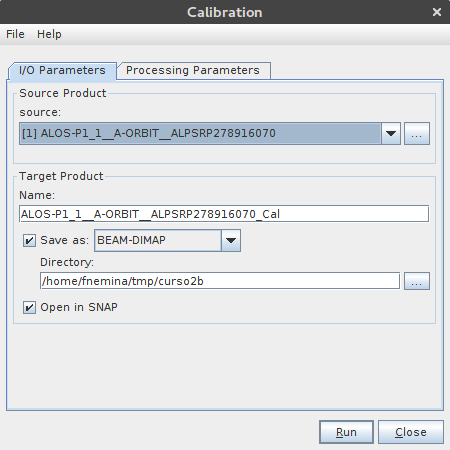
\includegraphics[width=0.35\textwidth]{fig:calibrar1.png}}
    \hfill
    \subfloat[Processing parameters]{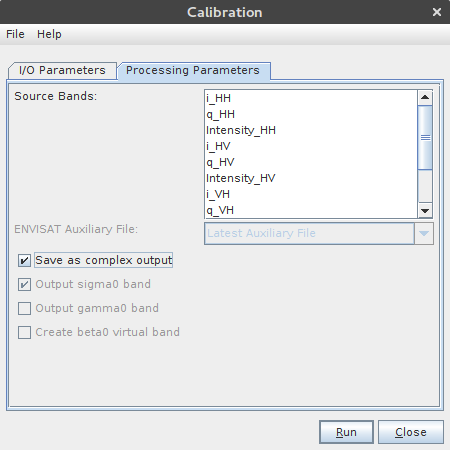
\includegraphics[width=0.35\textwidth]{fig:calibrar3.png}}
    \caption{}
    \label{fig:calibrar}
\end{figure}

\subsection{Calculo de matriz de coherencia}

Para calcular la matriz de coherencia, una vez calibrada la imagen, utilice la herramienta \menu{Radar>Polarimetric>Polarimetric matrix generation}.

Seleccione la imagen \directory{ALOS-P1\_1\_\_A-ORBIT\_\_ALPSRP278916070\_Cal} y en Processing parameters elija la matrix T3. Por el momento, no se preocupe por el significado de esta matriz (Figura \ref{fig:t3}).

\begin{figure}[h!]
    \centering
    \subfloat[I/O Parameters]{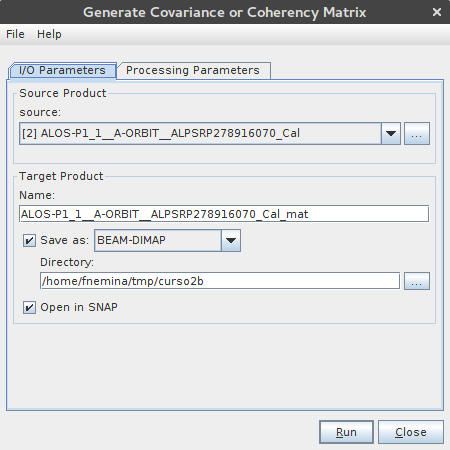
\includegraphics[width=0.35\textwidth]{fig:t31.png}}
    \hfill
    \subfloat[Processing parameters]{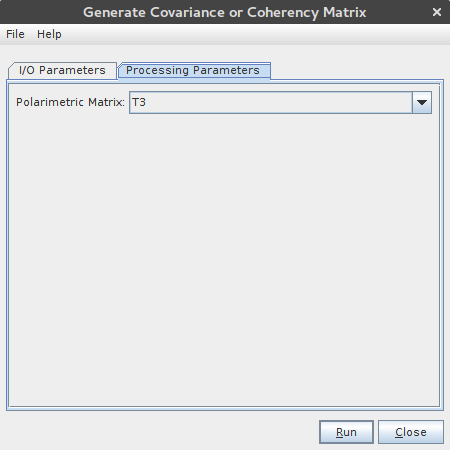
\includegraphics[width=0.35\textwidth]{fig:t32.png}}
    \caption{}
    \label{fig:t3}
\end{figure}

\subsection{Filtrado}

En el caso de imágenes full polarimetricas se pueden aplicar distintos tipos de filtros, que se encuentran en el menu \menu{Radar>Polarimetric>Polarimetric speckle filter}. Utilice en este caso el filtro \menu{Refined Lee} sobre la imagen \directory{ALOS-P1\_1\_\_A-ORBIT\_\_ALPSRP278916070\_Cal\_mat} (Figura \ref{fig:plee})

\begin{figure}[h!]
    \centering
    \subfloat[I/O Parameters]{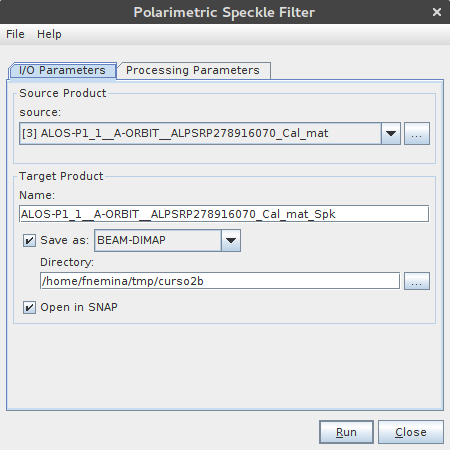
\includegraphics[width=0.35\textwidth]{fig:plee1.png}}
    \hfill
    \subfloat[Processing parameters]{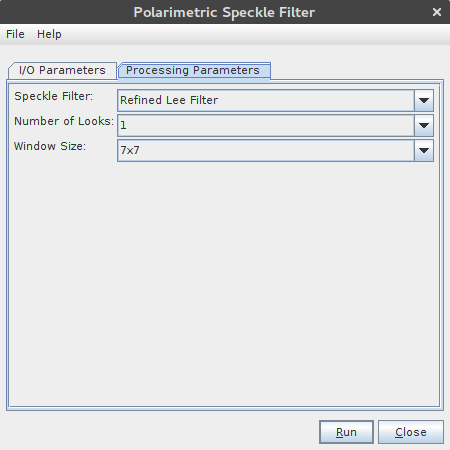
\includegraphics[width=0.35\textwidth]{fig:plee2.png}}
    \caption{}
    \label{fig:plee}
\end{figure}

\subsection{Proyección}

Reproyecte la imagen en el terreno aplicando los procesos de \emph{Deskewing} sobre un modelo de elevación digital.

\section{Descomposición de Pauli}

La descomposición de Pauli permite separar la información sobre interacciones de tipo doble rebote, en volumen y especulares, en una imagen full polarimétrica

La descomposición genera tres canales que suelen interpretarse de la siguiente manera:

\begin{itemize}
    \item Rojo: Información por procesos de un solo rebote o un número impar par de rebotes.
    \item Verde: Información por procesos de scatering en volumen.
    \item Azul: Información por procesos de doble rebote o un número par de rebotes.
\end{itemize}

Obtenga la descomposición de Pauli usando la herramienta \menu{Radar>Polarimetric>Polarimetric Decomposition} seleccionando como entrada la imagen corregida en terreno y la descomposición la de Pauli en Processing parametric(Figura \ref{fig:pauli})

\begin{figure}[h!]
    \centering
    \subfloat[I/O Parameters]{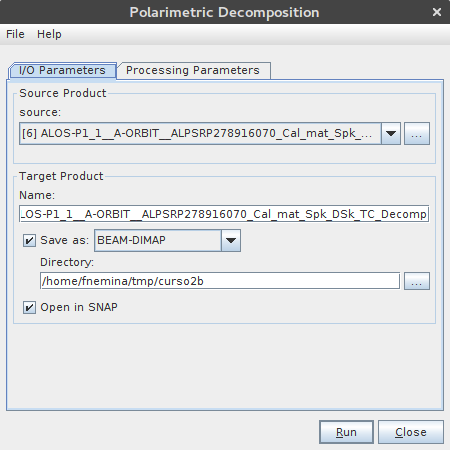
\includegraphics[width=0.35\textwidth]{fig:pauli1.png}}
    \hfill
    \subfloat[Processing parameters]{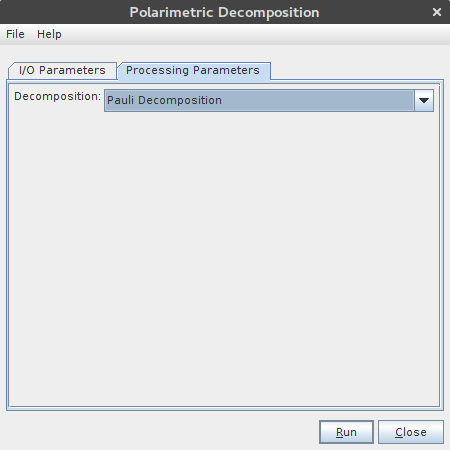
\includegraphics[width=0.35\textwidth]{fig:pauli2.png}}
    \caption{}
    \label{fig:pauli}
\end{figure}

Observe los resultados haciendo click derecho sobre la imagen obtenida en la opción \emph{Open RGB image window} (Figura \ref{fig:pauli}).

\begin{figure}[h!]
    \centering
    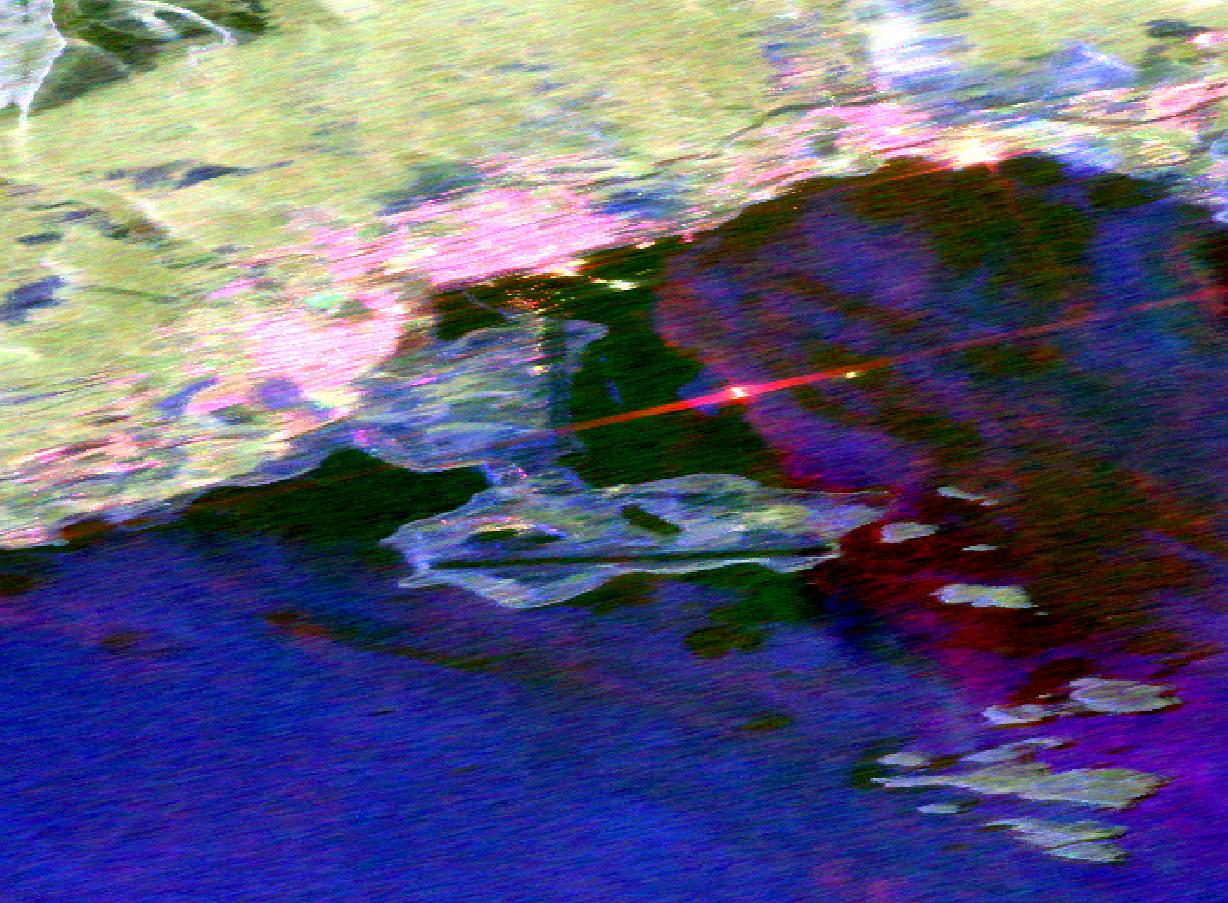
\includegraphics[width=0.7\textwidth]{fig:pauli.jpg}
    \caption{}
    \label{fig:pauli}
\end{figure}

\section{Actividades}
En la descomposición de Paulin:
\begin{que}
    ¿De qué color  se observan:
\begin{itemize}
  \item las zonas urbanas
  \item los bosques
  \item el agua
  \item la pista de aterrizaje
\end{itemize}

\end{que}
